\documentclass[11pt]{scrartcl}
\usepackage{graphicx}

\begin{document}
\section{Dokumentation}

\subsection{Client}

\subsubsection{Bedienung}

\begin{itemize}
	\item Die datei 'index.html' mit dem Browser \"offnen
	\item Zeitintervall und Messdauer wählen
	\begin{itemize}
		\item Optional kann auch ein Minimal- und Maximalwert gew\"ahlt werden, bei dessen unter- bzw. \"uberschreitung eine Warnung ausgegeben wird.
	\end{itemize}
	\item Zum starten der Messung auf den Button 'Start' klicken
	\item Die Messwerte der aktuellen Sitzung k\"onnen jederzeit \"uber den Button 'Save CSV' lokal auf dem Computer gespeichert werden
	\item Zum stoppen der Messungen den Button 'Stopp' klicken
	\begin{itemize}
		\item Achtung: Nach dem erneuten start der Messungen gehen nicht gespeicherte Daten verloren!
	\end{itemize}
\end{itemize}

\subsubsection{Systemvoraussetzungen}

\begin{itemize}
	\item Der Client kann eine Netzwerkverbindung zum Server herstellen
	\item Zur Verwendung des Clients muss einer der folgenden Browser mit aktiviertem Javascript verwendet werden
	\begin{itemize}
		\item Desktop:	
		\begin{itemize}
			\item Firefox (4+)
			\item Internet Explorer (10+)
			\item Chrome (10+)
			\item Safari (5.1+)
			\item Opera (11.64+)
		\end{itemize}
		\item Mobile:	
		\begin{itemize}
			\item Android (4.0+)
			\item BlackBerry OS (10+)
			\item Chrome Mobile (25+)
			\item Firefox Mobile (16+)
			\item Safari (5.1+)
			\item Opera Mobile (12.00+)
			\item Windows Phone 7 (8+)
		\end{itemize}
	\end{itemize}
\end{itemize}

Client (Firefox)\\

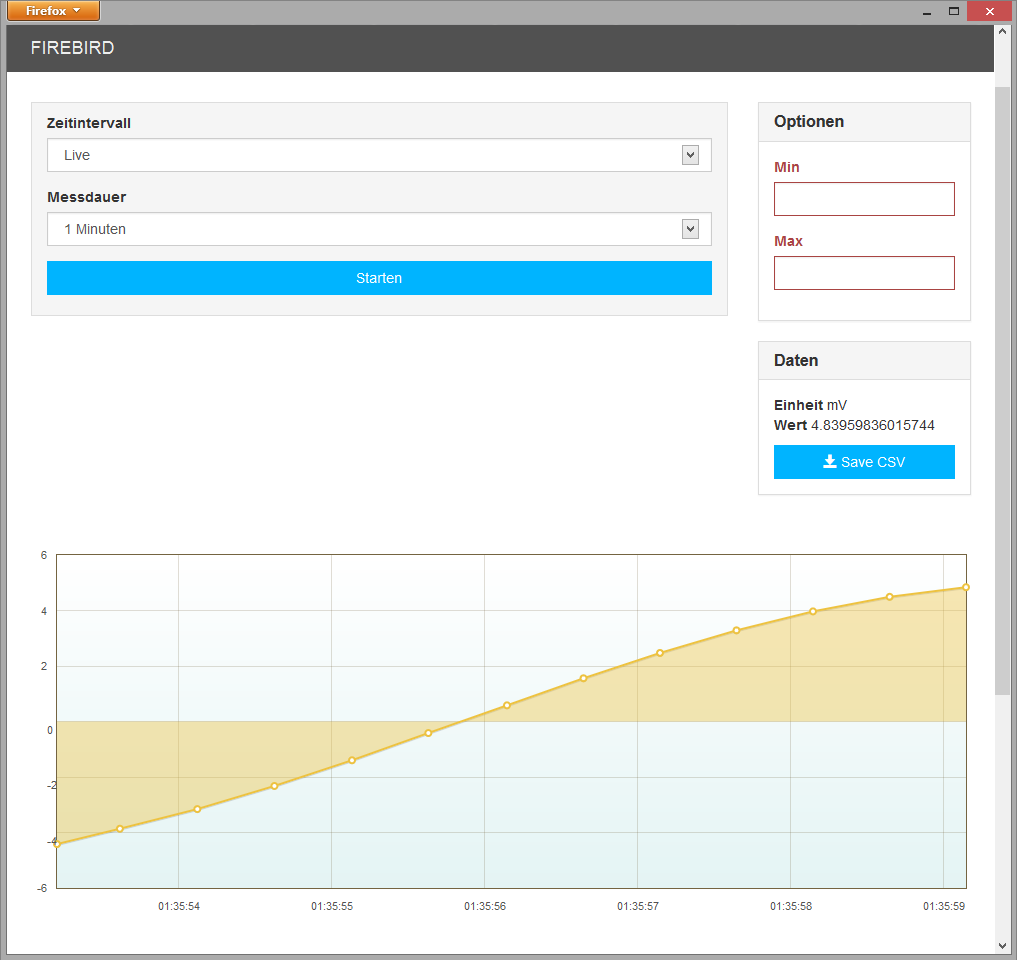
\includegraphics[width=\textwidth]{Desktop}
\pagebreak

\subsection{Server}

\subsubsection{Bedienung}

\begin{itemize}
	\item Zum starten des Servers die Anwendung 'metexsrv.exe' \"offnen
	\begin{itemize}
		\item Es stehen folgende optionale Parameter zur verf\"ugung:
		\begin{itemize}
			\item '-t' Aktiviert den Testmodus. Es ist kein Messger\"at erforderlich
			\item '-i port' Setzen des COM-Port (Standard 'COM1')
			\item '-p port' Setzen des Server-Port (Standard '12345')
		\end{itemize}
	\end{itemize}
	\item Nach dem starten der Anwendung kann der Client bedient verwendet werden.      Mit einem beliebigen Tastendruck in der Konsole wird die Serveranwendung beendet.
	\item Wird eine neue Verbindung zu einem Client aufgebaut, oder eine vorhandene getrennt, wird ein Meldung in der Konsole ausgegeben
\end{itemize}

Server \\

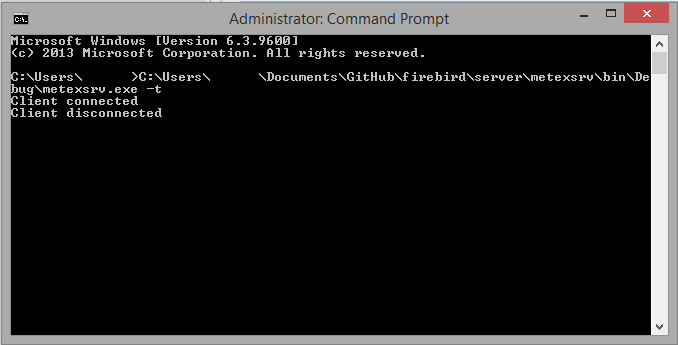
\includegraphics[width=\textwidth]{Konsole}

\end{document}